 \documentclass[11pt]{amsart}

\RequirePackage[OT1]{fontenc}

\usepackage{biblatex}
%\bibliographystyle{apalike}


\usepackage{tchdr}
\boldshortcuts

\usepackage{graphicx}
\usepackage{wrapfig}
\usepackage{setspace}
\DeclareGraphicsExtensions{.eps, .ps}
\usepackage{soul,color,hyperref}
\usepackage{amsmath, amsthm, amsfonts}
\usepackage[margin=1.5in]{geometry}

% \numberwithin{equation}{section}
% \theoremstyle{plain}
% \newtheorem{theorem}{Theorem}[section]
% \newtheorem{example}{Example}
% \newtheorem{remark}{Remark}
% \newtheorem{corollary}[theorem]{Corollary}
% \newtheorem{criterion}[theorem]{Criterion}
% \newtheorem{definition}[theorem]{Definition}
% \newtheorem{exercise}[theorem]{Exercise}
% \newtheorem{lemma}[theorem]{Lemma}
% \newtheorem{proposition}[theorem]{Proposition}

\def\pr{\text{pr}}
\def\sgn{\text{sgn}}
\def\I{\bf I}

\begin{document}
\title[The Hypothesis of Testing]{The Hypothesis of Testing: Paradoxes arising out of reported coronavirus case-counts}
% \author{Walter Dempsey\thanks{Department of Biostatistics, University of Michigan, 1415 Washington Heights, U.S.A. E-mail: wdem@umich.edu}}
\maketitle

\begin{abstract}
Many statisticians, epidemiologists, economists and data scientists have registered serious reservations regarding the reported coronavirus case-counts. Limited testing capacity across many states has been widely identified as a key driver of suppressed coronavirus case-counts.  Calls for increased testing capacity are well-justified and increasingly frequent.  While expanded testing is a laudable goal, selection bias will impact estimates of disease prevalence and the effective reproduction number until the entire population is sampled.  Moreover, tests are imperfect.  False positive/negative rates interact in complex ways with selection bias.  This note attempts to clarify this interaction.  Through simple calculations, we demonstrate pitfalls and paradoxes that can arise when considering case-count data in the presence of selection bias and measurement-error. The discussion guides a series of suggestions to improve current case-count reporting.
\end{abstract}

\section{Introduction}
The World Health Organization has declared the coronavirus disease 2019 (COVID-19) a public health emergency.  As of April 27th, 2020, a total of 2,993,00 cases have been confirmed worldwide.  As of that afternoon, the New York Times reports at least 965,214 people across the United States have tested positive for the virus, and at least 49,465 patients with the virus have died.  Aggressive policies had been put in place across the US with at least 50\% of the US population officially urged to stay home via state-wide executive actions.

Despite these necessary steps, the data landscape for understanding COVID-19 remains limited.  Public databases maintained by Johns Hopkins University (\url{https://bit.ly/2UqFSuA}) and the New York Times (\url{https://bit.ly/2vUHfrK}) provide incoming county-level information of confirmed cases and deaths.  Statisticians, epidemiologists, economists, and data scientists the world over have been using this granular data to build model-based forecasts of future COVID-19 case-counts, deaths, and hospitalizations.  Variations on the SIR models have been used to draw inferences and build forecasts.  In most cases, parameter inference uses observed case-count and/or observed COVID-19 related deaths to infer latent trajectories of the pandemic (cites).

The goal of this paper is to express reservations at the use of case-counts as a proxy for prevalence and disease trajectory as well as its use as direct input into estimation of standard epidemiological models for inference and forecasting.  The reason is simple: current models ignore selection bias and measurement-error.

Selection bias enters due to differences in testing strategies across countries and states.  In the US, for example, limited testing capacity has caused local and state health departments to focus on testing only  high-risk populations.  Testing requires the individual to self-select into testing.  Demands for testing increases, while laudable, ignore the issues of self-selection and measurement-error. While increasing testing capacity increases data quantity, there is no guarantee for increased data quality.  We will show that aggressive pushes for ramped up testing capacity that are tied to decreases in data quality may have a deleterious effect in our ability to estimate quantities of interest such as prevalence and effective reproduction number.

In this paper, we will demonstrate the complex interaction between these two fundamental concepts.  Measurement-error is often associated with parameter attenuation; howeve,r we show that the combination with selection effects can cause bias in parameter estimates to change sign and increase/decrease in magnitude.  Moreover, the bias may depend on the sampling fraction, prevalence, and population size.  Without a complete understanding of these interations, we are destined to misinterpret case-counts and come to erroneous conclusions.   We will show, through simple calculations, how we can misguide ourselves and the need for more precision and care in presenting COVD-19 statistical models to the broader research and non-academic communities.

\subsection{Related work}

There has been an abundance..

However, most complain about testing \emph{capacity} (cite Nate Silver), there is clearly issues of data quality.

Measurement-error discussions.
Selection bias . Proponents of this critique suggest well-designed studies.

Stanford study was Ionides.  They however, forgot about Critique \#2: measurement

\subsection{Outline}

This article discusses the relationship between three statistical concepts: selection bias, measurement-error, and the long-forgotten population size. We clarify mathematically why the situation is much more complex than it first appears.  Through simple mathematical argument, we demonstrate five important, yet often forgotten, tenants of statistical science.  First we show that unadjusted prevalence rates are unsurprisingly biased when tests are imperfect. What is surprising is that the direction and magnitude of the bias can vary substantially and interacts with the sampling fraction.  Next we show that data quality for adjusted prevalence rates incorporate an additional term in the error decomposition that highlights the interplay among measurement error, selection bias, and prevalence.  Third, we show that daily trends in rate of positive tests is equally problematic even if testing rates and selection protocols are held constant.  We show that the rate of change in COVID-19 observed case-counts are often an underestimate of the true rate. This implies use of observed rates will lead a data analyst to be overly optimistic in the early stages that the disease is not an issue, and also overly optimistic in the decline of the prevalence after the peak.   Fourth, we show that estimates of the reproducility rate are also impacted.

The above analyses are focused on the issues with using observed case-counts to understand the trajectory for a single country or state.  The media and organizations are also interested in comparisons of case-counts across countries. To account for population size, case-counts are scaled by the country population size.  We show that even after this adjustment, cross-country comparisons can be plagued by estimation error scaling by population size.  We end the paper with a discussion of the benefits of randomized testing, where auxiliary information is most relevant, and the distinction between data quality and decision making in the current pandemic.

\section{Analysis of case-count data}

We start with some simple notation.  Let $N$ denote the population size.  For state-level analysis $N$ is the state's total population, while for country-level analysis $N$ is the country's total population.  At a fixed moment in time, let $Y_j$ denote COVID-19 status for the $j$th individual in the population, $j=1,\ldots, N$. Here, like in survey methodology (cite), we treat COVID-19 status as a fixed but unknown population quantity of interest. For simplicity, we start by ignoring the dynamic nature of the viral outbreak as well as the fact that individuals can recover from the disease and assume either individual $j$ is COVID-19 positive and $Y_j=1$ or is COVID-19 negative and $Y_j=0$. We also let $I_j \in \{0,1\}$ be an indicator that the individual was selected for testing ($I = 1$) or not ($I=0$).

To start, we assume the primary questions of interest are estimates of the overall number of COVID-19 cases and/or disease prevalence. That is, we are interested in either the population total $Y = \sum_{j=1}^N Y_j$ or the population average $\bar Y = Y/N$. Suppose that $n$ tests are performed and we observe the values $y_1, \ldots, y_n \in \{0,1\}$.  Then a natural candidate for prevalence is the proportion of positive tests $\bar y = \frac{1}{n} \sum_{i=1}^n y_i$, and a natural candidate for overall cases is $N \times \bar y$.
Under simple random sampling (SRS) or any other epsem design, the above are unbiased estimators of the population-level quantities of interest.  Under SRS, the variance of the estimator can be expressed as $\frac{1}{N-1} \times \frac{1-f}{f} \times \sigma_Y^2$ where $f = n/N$ is the sampling fraction and $\sigma_Y^2 = \frac{1}{N} \sum_{i=1}^N (Y_i - \bar Y)^2 = \bar Y (1- \bar Y)$.

When the sampling mechanism is non-random, selection effects may cause bias in the above estimates. To better understand this issue, Meng (2019) provided the following intuitive and powerful statistical decomposition of the error between $\bar y$ and the true proportion $\bar Y$
$$
\bar y_n - \bar Y =  \rho_{I, Y} \times \sqrt{\frac{1-f}{f}} \times \sigma_Y.
$$
The first term represents \emph{data quality}, the second \emph{data quantity}, and the third \emph{problem difficulty}. The term $\rho_{I,Y}$ is the empirical correlation between the population values~$\{ Y_j \}_{j=1}^N$ and the selection values $\{ I_j \}_{j=1}^N$.  Under simple random sampling, $E_{\I} [ \rho_{I,Y} ] = 0$, where the expectation is with respect to the selection mechanism~$\I$, so there is no bias.  The SRS variance formula above shows that $E_{\I} [ \rho_{I,Y}^2 ]  = 1/(N-1)$.  The key issue with selective testing is that $E_{\I} [ \rho_{I,Y} ] \neq 0$.  Meng identified this as the fundamental issue that can lead to paradoxes in the analysis of big data.

Here we highlight the core insights relevant to the COVID-19 crisis.  First, comparing the mean-squared error under selection mechanism $\I$ and SRS, we see that
$$
\frac{E_{\I} \left[ (\bar y_n - \bar Y)^2 \right]}{\sqrt{V_{SRS} (\bar Y)}} = (N-1) E_{\I} \left[ \rho_{I,Y}^2 \right].
$$
This points to a troubling and paradoxical situation: the error relative to SRS increases as a function of population size.  Meng terms this the ``Law of Large Populations'' (LLP).  The points to a critical issue in the current media practices in communication of case-count data: two countries with the same testing strategy (i.e., $\rho_{I,Y}$ equal) can yield wildly different estimates due to population size.  Large countries like the US may have similar true prevalence rates as smaller countries like the UK.  Even under similar testing strategies, the mean-squared error in the prevalence rate for the US will have substantially more variation.  For example, the MSE will be almost 5 times that in the US compared to the UK.  Therefore, strong opinions built from case-count records may be substantially distorted.

Second, there have been calls for increased testing.  While important, many conflate increased testing capacity with increased quality of testing.  We will discuss this point further in Section XX.  In the COVID-19 crisis, for example, New York has performed a total of $n = 872,481$ tests from April 20th to 30th.  In Figure XX, we present the trajectory of testing per day and positive cases per day.  The New York population is $N=8,399,000$; removing those individuals who have been already tested leaves a population of $7,XXX,XXX$.  This leads to a fraction sampled of $f = 0.1$.  A recent study attempted to estimate prevalence in New York.  After appropriate adjustments (see Appendix XX for details), a plausible range for prevalence seems to be between $2\%$ and $12\%$.  Suppose that individuals who are COVID-19 positive are $1.5$ times more likely to get tested than those individuals who are COVID-19 negative (a modest relative rate).  The question is ``What is the sample size from a SRS that would yield equivalent MSE in the estimated prevalence?'' Using the above MSE result, Meng showed the effective sample size is equal to $n_{eff} \leq \frac{1}{E_I [ \rho_{I,Y}^2 ]} \frac{f}{1-f}$ and that ranges from $208$ to $38$ across the range of plausible values of prevalence.  This is the sad state of affairs, saying that the effective sample size even in best case scenarios is not better than a small random sample from the population.

The remainder of this paper aims to build upon these fundamental insights by extending the decomposition in two directions: accounting for  measurement-error and the temporal nature of the pandemic.  We then discuss testing strategies, effective sampling methods, and data versus decision-making.

\subsection{Imperfect testing}

Tests are imperfect.  COVID-19 testing is no exception. Here we investigate the interplay between imperfect testing and selection bias.  When discussing testing inaccuracies, the standard assumption is measurement-error leads to parameter attenuation.  When paired with selection bias, however, the two sources of error become entangled, and the biases can become magnified, muted, or even switch signs.

First we require some additional notation.  Let $P_j$ be an indicator of measurement error, equal to $1$ when we mismeasure the outcome and $0$ when we observe the true outcome. We suppose this is a stochastic variable that satisfies $\pr(P_j = 1 \mid Y_j = 1) =: FN$ is the false-negative rate and $\pr(P_j = 1 \mid Y_j = 0) =: FP$ is the false-positive rate.  If individual $j$ is selected (i.e., $I_j = 1$) then the observed outcome can be written as $Y_j^\star = Y_j(1-P_j) + (1-Y_j) P_j$.  Suppose disease prevalence was estimated as the fraction who tested positive for COVID-19, i.e., $\bar y_n^\star = \frac{\sum_{i=1}^N I_j Y_j^\star}{\sum_{i=1}^N I_j}$.  We can again investigate the error compared to the true prevalence $\bar Y$ in statistical terms:
$$
\bar y_n^\star - \bar Y = \sqrt{\frac{1-f}{f}} \left[ \rho_{I,Y} \times \sigma_Y + \rho_{I,PZ} \times \sigma_{PZ} + \sqrt{\frac{f}{1-f}}  \left( FP - (FP+FN) \bar Y \right) \right] .
$$
where $Z = 1-2Y$. The first term represents the perfect testing regime, the second term represents the interaction between imperfect testing and selection bias, while the third time represents the bias due to imperfect testing.  From here on, we refer to $\rho_{I,Y}$ as the \emph{true data quality}, and $\rho_{I,PZ}$ as the \emph{observed data quality} that accounts for both selection bias and measurement-error.  We show the sign of $\rho_{I,PZ}$ is the opposite of the sign of $\rho_{I,Y}$, and so the second term adjusts the true data quality.

We start by considering the first two terms and assess whether the sign of the bias can reverse due to the interaction of measurement-error and selection bias.  To do this, we require the sampling rates differential.  Let $f_1 := \pr (I_J = 1 \mid Y_J = 1)$ and $f_0 := \pr(I_J = 1 \mid Y_J = 1)$ be the sampling rates.  Then $\Delta = f_1 - f_0$ is the sampling rate differential and we have
$$
\rho_{I,Y} \times \sigma_Y + \rho_{I,PZ} \times \sigma_{PZ} =
\rho_{I,Y} \times \sigma_Y \left[ 1 - \Delta \times \frac{\bar Y}{1-\bar Y} \times \frac{FP(1-\bar Y) + FN \cdot \bar Y}{f_0 (1-\bar Y) + f_1 \bar Y} \right].
$$
The final term in brackets is the \emph{measurement-error adjustment to data quality} which is a complex function of sampling rate differential, the odds ratio, and the ratio of measurement-error interaction with prevalence and sampling rates interaction with prevalence. Note $\sgn(\Delta) = \sgn(\rho_{I,Y})$ by equation~\ref{eq:binaryrho} so the measurement-error adjustment either shrinks the data quality measure toward zero or reverses its sign.

While prior investigations have noted the interaction between measurement-error and selection bias (cites), the interaction with the sample size relative to the population, i.e., $f$, has largely been ignored.  The above statistical decomposition clarifies the importance of this quantity~$f$.  In particular, note that the statistical error also includes a bias term due to measurement-error and this term increases as the sampled fraction $f$ increases. Therefore, how the first two terms interact with the final term depends on the fraction of the population sampled.  This interaction is complex, but implies that whether the estimate $\bar y^\star_n$ is an overestimate or underestimate is a complicated question due to the relation amongst these three pieces.


In the current setting, supposing the ratio of conditional selection rates $f_1/f_0$ is equal to 1.5.  The false negative rate ranges from 15\% to 40\%, while the false positive rate is low (around 1\%). Then under plausible prevalence rates that we discussed before, the relative MSE ranges from 1.4 to 0.12.  So that means in some cases we have a huge increase in MSE and in other settings we have a huge decrease in MSE.  What drives this is the false negative rate interaction with prevalence and sampling rates.  Therefore, whether we are better or worse off is a very difficult question to answer.


The attentive data analyst will recognize the estimator $\bar y_n$ is biased even for simple random samples and, if sensitivity and specificity were known a priori, may suggest the alternative estimator $\tilde y_n = \bar y_n + (1-\bar y_n) FP + FN \bar y_n$ which is unbiased under simple random sampling. We again wish to express the error $\tilde  y_n - \bar Y$ in statistical terms. In the appendix, we show that the error now can be expressed as
$$
\tilde y_n - \bar Y = \rho_{I,Y} \times \sqrt{\frac{1-f}{f}} \times \sigma_{Y}
\times \underbrace{\left[ 1 + FP + FN - \Delta \times \frac{\bar Y}{1-\bar Y} \times \frac{FP(1-\bar Y) + FN \cdot \bar Y}{f_0 (1-\bar Y) + f_1 \bar Y} \right]}_{D_M}.
$$
The first term is the same as before but increased by $(1 + FP + FN)$ to account for the additional uncertainty due to measurement-error.  The second term is the interaction between selection bias and measurement error.  Interestingly we can show that the sign is reversed, i.e., $sgn(\rho_{I,PZ}) = 1 - sgn(\rho_{I,Y})$, leading to an absolute \emph{reduction} in the error.

For this adjusted estimate, we can see that the directionality is maintained.  Therefore, the benefit is if the expected correlation is positive, we can feel like the estimate is likely an over-estimate and vice versa.  You pay a penalty in terms of variance and therefore the MSE may not be much smaller (CHECK!)

Under the same numbers, $D_M$ is approximately 1.7.  The effective sample size can then be bounded by
$$
n_{eff} = \frac{f}{1-f} \times \frac{1}{E_{I} \left[ \rho_{I,Y}^2 D_M^2 \right]}.
$$
This lowers the ranges by a factor of almost $3$, leading to effective sample sizes from 69 to 13.

The above argument shows that the effective sample size is affected in a complex manner by the interaction between selection bias and measurement error.  Here, we discuss the impact of the interaction on the effective sample size when testing capacity is tied to measurement-error.  In the current pandemic, there have been well-justified calls for increases in testing capacity.  These increases, however, may come at the cost of increases in false-positive and false-negative rates.  In terms of effective sample size, if the data quality term remains constant, then testing increases can actually hurt effective sample size.  Consider the simplest case where $f$ increases from $0.05$ to $0.1$; suppose this required including tests such that the false negative rate jumps from $0.05$ to $0.15$.  Then we would think effective sample size should increase by a factor of $3.4$ but the actual increase is by a factor of only $1.8$!  Think about what this is saying, this is saying that sampling $15\%$ of the population rather than $5\%$ will only increase the effective sample size by a factor $1.8$ if the selection-bias persists and the false negative rate climbs to $15\%$.   It has been reported that false negative rates could increase more than that (cite NYT) and the false positive rate could go up slightly as well.  In a worst case scenario, if $FN \to 0.3$ and $FP \to 0.05$ then the factor is only 1.3.

\begin{wrapfigure}{r}{0.5\textwidth}
\centering
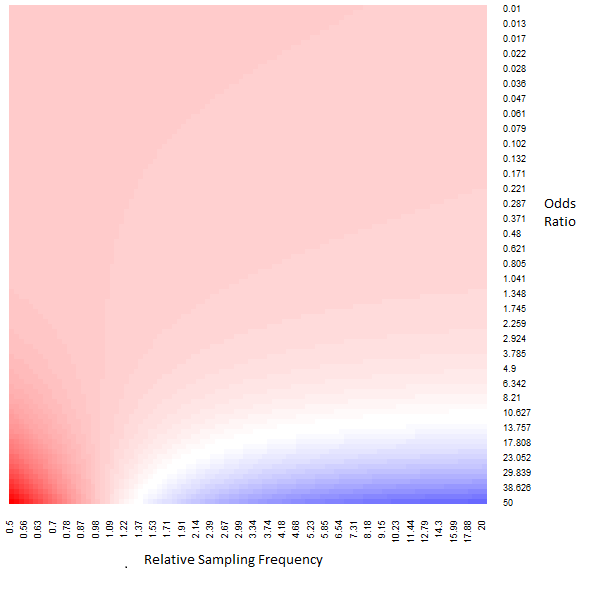
\includegraphics[width = 0.4\textwidth]{../methods/figs/mem_heatmap_article.png}
\caption{Measurement-error data quality adjustment: relative frequency $f_1/f_0$ (x-axis) against odds ratio (y-axis) for $FP=0.15$ and $FN=0.10$. Color scaled so blue = $-6$, white = 0, and red = $6$.}
\vspace{-0.3cm}
\end{wrapfigure}

\subsection{Regrettable rates: complex biases resulting from self-selection}
\label{section:rates}

The data analyst, now frustrated with me but at least wary of estimating prevalence and total counts, pauses and thinks.  They return shortly thereafter, a bit agitated but persistent: \emph{Ok, perhaps total counts is a lost cause. Certainly, however, we can estimate the rate of growth.  All I want to know is when we hit the point at which the curve flattens and number of deaths decrease.  That can't be too hard, surely!}

Unfortunately, ratio estimators do not cancel errors as now both the numerator and the denominator are uncertain.  This means selection bias and measurement error can have paradoxical effects.  Here we consider the ratio estimators for the relative change in the prevalence rate.  We let $\bar Y_{t-1}$ and $\bar Y_{t}$ denotes the prevalence at time step $t-1$ and $t$ respectively (i.e., prevalence on two consecutive days).  Then the ratio estimator is given by $r = \bar y_t / \bar y_{t-1}$.  We assume both numerator and denominator are the prevalence estimates adjusted for measurement-error. If the sample size at each time were equal (i.e., $n_1 = n_2 = n$) then this analysis would be equivalent to comparing the increase in observed case-counts (i.e., $\bar y_t/\bar y_{t-1} = y_t/y_{t-1}$).  We wish to express the error $\frac{\bar y_t}{\bar y_{t-1}} - \frac{\bar Y_{t}}{\bar Y_{t-1}}$ in statistical terms.  Using a Taylor series approximation, we show that the error can be expressed approximately as
$$
\begin{aligned}
\frac{\bar Y_t}{\bar Y_{t-1}} &\times \bigg[ \rho_{I_t,Y_t} D_{M_t} \sqrt{\frac{1-f_t}{f_t}} CV (Y_t)  -\rho_{I_{t-1},Y_{t-1}} D_{M_{t-1}} \sqrt{\frac{1-f_{t-1}}{f_{t-1}}} CV (Y_{t-1}) \bigg] \\
&\times \left[ 1 - \rho_{I_{t-1},Y_{t-1}} D_{M_{t-1}} \sqrt{\frac{1-f_{t-1}}{f_{t-1}}} CV (Y_{t-1}) \right]
\end{aligned}
$$
where $\rho_{I_j, Y_j}$ is the data quality, $f_j$ is the sampling fraction, $D_{M_j}$ is the measurement-error adjustment, and $CV(Y_j) = \sigma_{Y_j}/\bar Y_j$ is the coefficient of variation at time step $j$.  The magnitude of the error depends on the population-level ratio $\bar Y_{t-1} / \bar Y_{t-1}$ so a large decrease in the prevalence rate will have a relatively small error as compared to a large increase in the prevalence rate. The second term represents the ``cancellation'' that the naive analyst is hoping will occur.  The analyst's intuition only holds when the difference is equal to zero.  This occurs at times when data quality, sampling fraction, measurement-error, and prevalence are all held constant.  In the case of New York, for example, recent weeks it seems plausible that $\Delta$ (i.e., selection bias) has not changed drastically.  Figure XX shows the rate of testing remains constant and the total cases relative to the population is small enough such that $f_t \equiv f_{t-1}$ is reasonable. Finally, the measurement-error adjustment is likely to be constant as no new testing procedures have been reported (as far as this author knows).  We will show how such a setting leads to over-estimation prior to and under-estimation after peak prevalence.  The final component is an adjustment to this differential error based on the statistical error at the first time point.

Figure XXa shows a trajectory of bias under several prevalence and data quality scenarios.  We generate data from an SIR model with infection rate $\beta = XX$, total population = $100,000$.  We estimate the bias under a range of values for the relative sampling fraction $f_1/f_0$ and a sampling fraction of $f = 0.05$.  Figure XXb shows the trajectory of $\bar Y_t / \bar Y_{t-1}$.  We see that in each case, the rate of change in prevalence is overestimated prior to the peak and then underestimated afterwards.  From a decision making perspective, such biases have impacts.  First, the over-estimation may give lawmakers and governors more leverage in proposing aggressive actions that reduce prevalence.  Of course, the analysis supports the argument that the estimates based on available data are overly pessimistic. What both sides miss is that the direction of bias is non-constant over time.  After we hit the peak, estimates will under-estimate prevalence.  Lawmakers and governors will be put under pressure to relax social distancing measures.  This will drive a sequence of cycle of panic and .

Moreover, the question is ``Can we trust the observed data to let us know if we have reached the peak?''  It appears that the peak time is the easiest to estimate in terms of having minimal error using availability data.  Note, however, that the standard errors on such estimates will be incredibly wide as the effective sample size is quite small compared to SRS at each time.  \textcolor{red}{Short description of effective sample size}.

\subsubsection{Estimation of effective reproduction number}
Many well-respected epidemiologists argue that tracking the effective reproduction number $R_t$ is the only way to manage through the crisis (cites).  We show here how these estimates are also impacted by selection bias and measurement error.  For simplicity, we again assume the estimates are adjusted for known false positive and false negative rates. Luis and Ribeiro (2008) show that under a Poisson likelihood, a simple relation between the trajectory of \emph{true new cases} and the effective reproduction number can be derived (see Appendix XX for discussion).  In particular, under an SIR model, the number of case counts on day $t$ is Poisson distributed with rate $K_{t-1} \exp \left( \frac{1}{\gamma} (R_t - 1) \right)$ where $K_{t-1} = Y_{t-1}-Y_{t-2}$ is the number of new cases on day $t-1$ and $\gamma$ is the serial interval which is approximately $7$ days for COVID-19 (Sanche, 2020).  Using this, a method of moments estimator of the effective reproduction number at time $t$ can be given by
$$
R_t = 1 + \frac{1}{\gamma} \log \left( \frac{K_t}{K_{t-1}} \right).
$$
Of course, we do not observe $K_t$ and $K_{t-1}$ but noisy proxies $y_t$ and $y_{t-1}$, i.e., the observed case-count on day $t$ and $t-1$ respectively. The hope is that $y_t/y_{t-1}$ is a good proxy for $K_t/K_{t-1}$. Let $\hat R_t = 1 + \frac{1}{\gamma} \log \left( y_t / y_{t-1} \right)$ be the estimated effective reproduction number on day $t$.  Under SRS with the same sample size at each step, this is true for sufficiently large sample size.  However, similar to Section~\ref{section:rates}, the proxy has error in both numerator and denominator that may cause issues.  We again wish to express the statistical error of $\hat R_t - R_t$ in useful terms.  We can re-arrange the error decomposition from Section~\ref{section:rates} to show that this error is given by
$$
\begin{aligned}
\frac{1}{\gamma}\log &\bigg( 1 + \bigg[ \rho_{I_t,K_t} D_{M_t} \sqrt{\frac{1-f_t}{f_t}} CV (K_t)  -\rho_{I_{t-1},K_t} D_{M_t} \sqrt{\frac{1-f_t}{f_t}} CV (K_t) \bigg] \\
&\times \left[ 1 - \rho_{I_t,K_t} D_{M_t} \sqrt{\frac{1-f_t}{f_t}} CV (K_t) \right] \bigg)
\end{aligned}
$$
So here we see the exact same trade-off as with the rates but on the logarithmic scale.  For small values $\log(1+x) = x$ so the biases are similar.  However, the error is no longer scaled by the rate of change in prevalence $\bar Y_2/\bar Y_1$. Instead the error is scaled by the serial interval $\gamma^{-1} = 1/7$.  Moreover, the error depends not on aggregate prevalence $\bar Y_t$ but fraction of new cases $\bar K_t$.

In Figure XXc, we show the error in this quantity.  The trajectory follows the same as before; however, the errors are....


\begin{figure}
\centering
\begin{subfigure}{.5\textwidth}
  \centering
  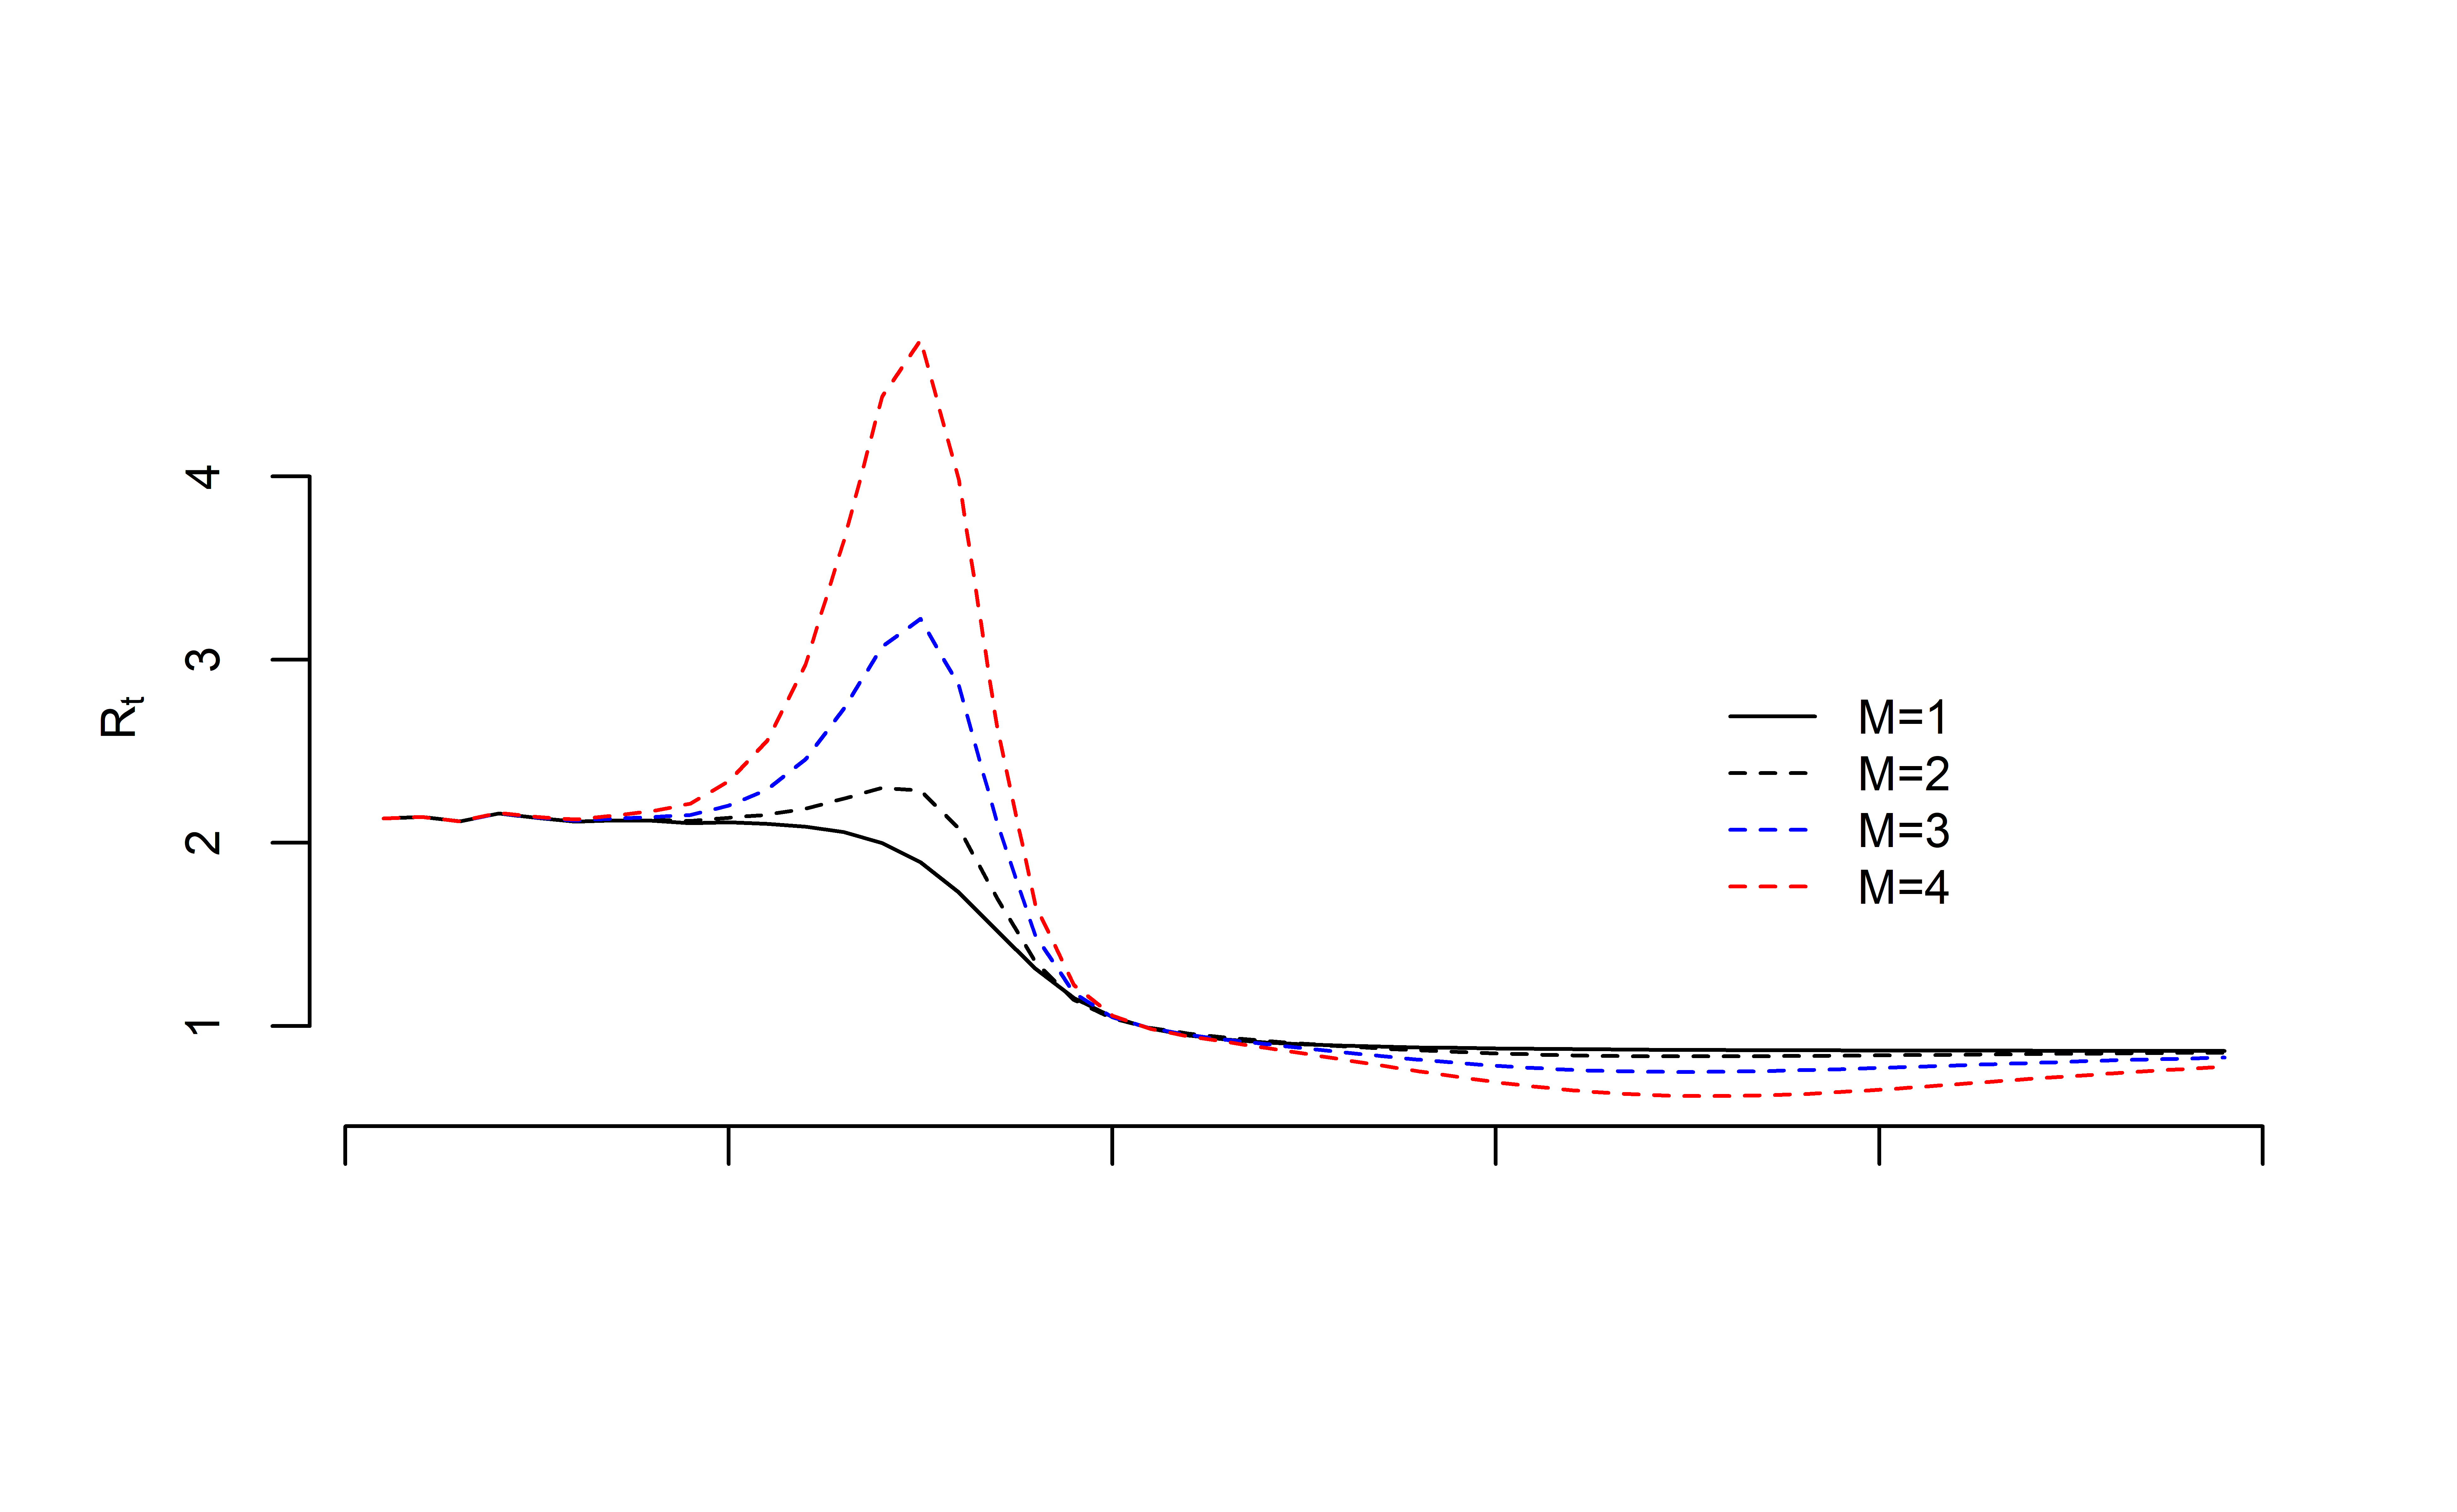
\includegraphics[width=.9\linewidth]{../methods/figs/sir_ratio.png}
  \caption{A subfigure}
  \label{fig:sub1}
\end{subfigure}%
\begin{subfigure}{.5\textwidth}
  \centering
  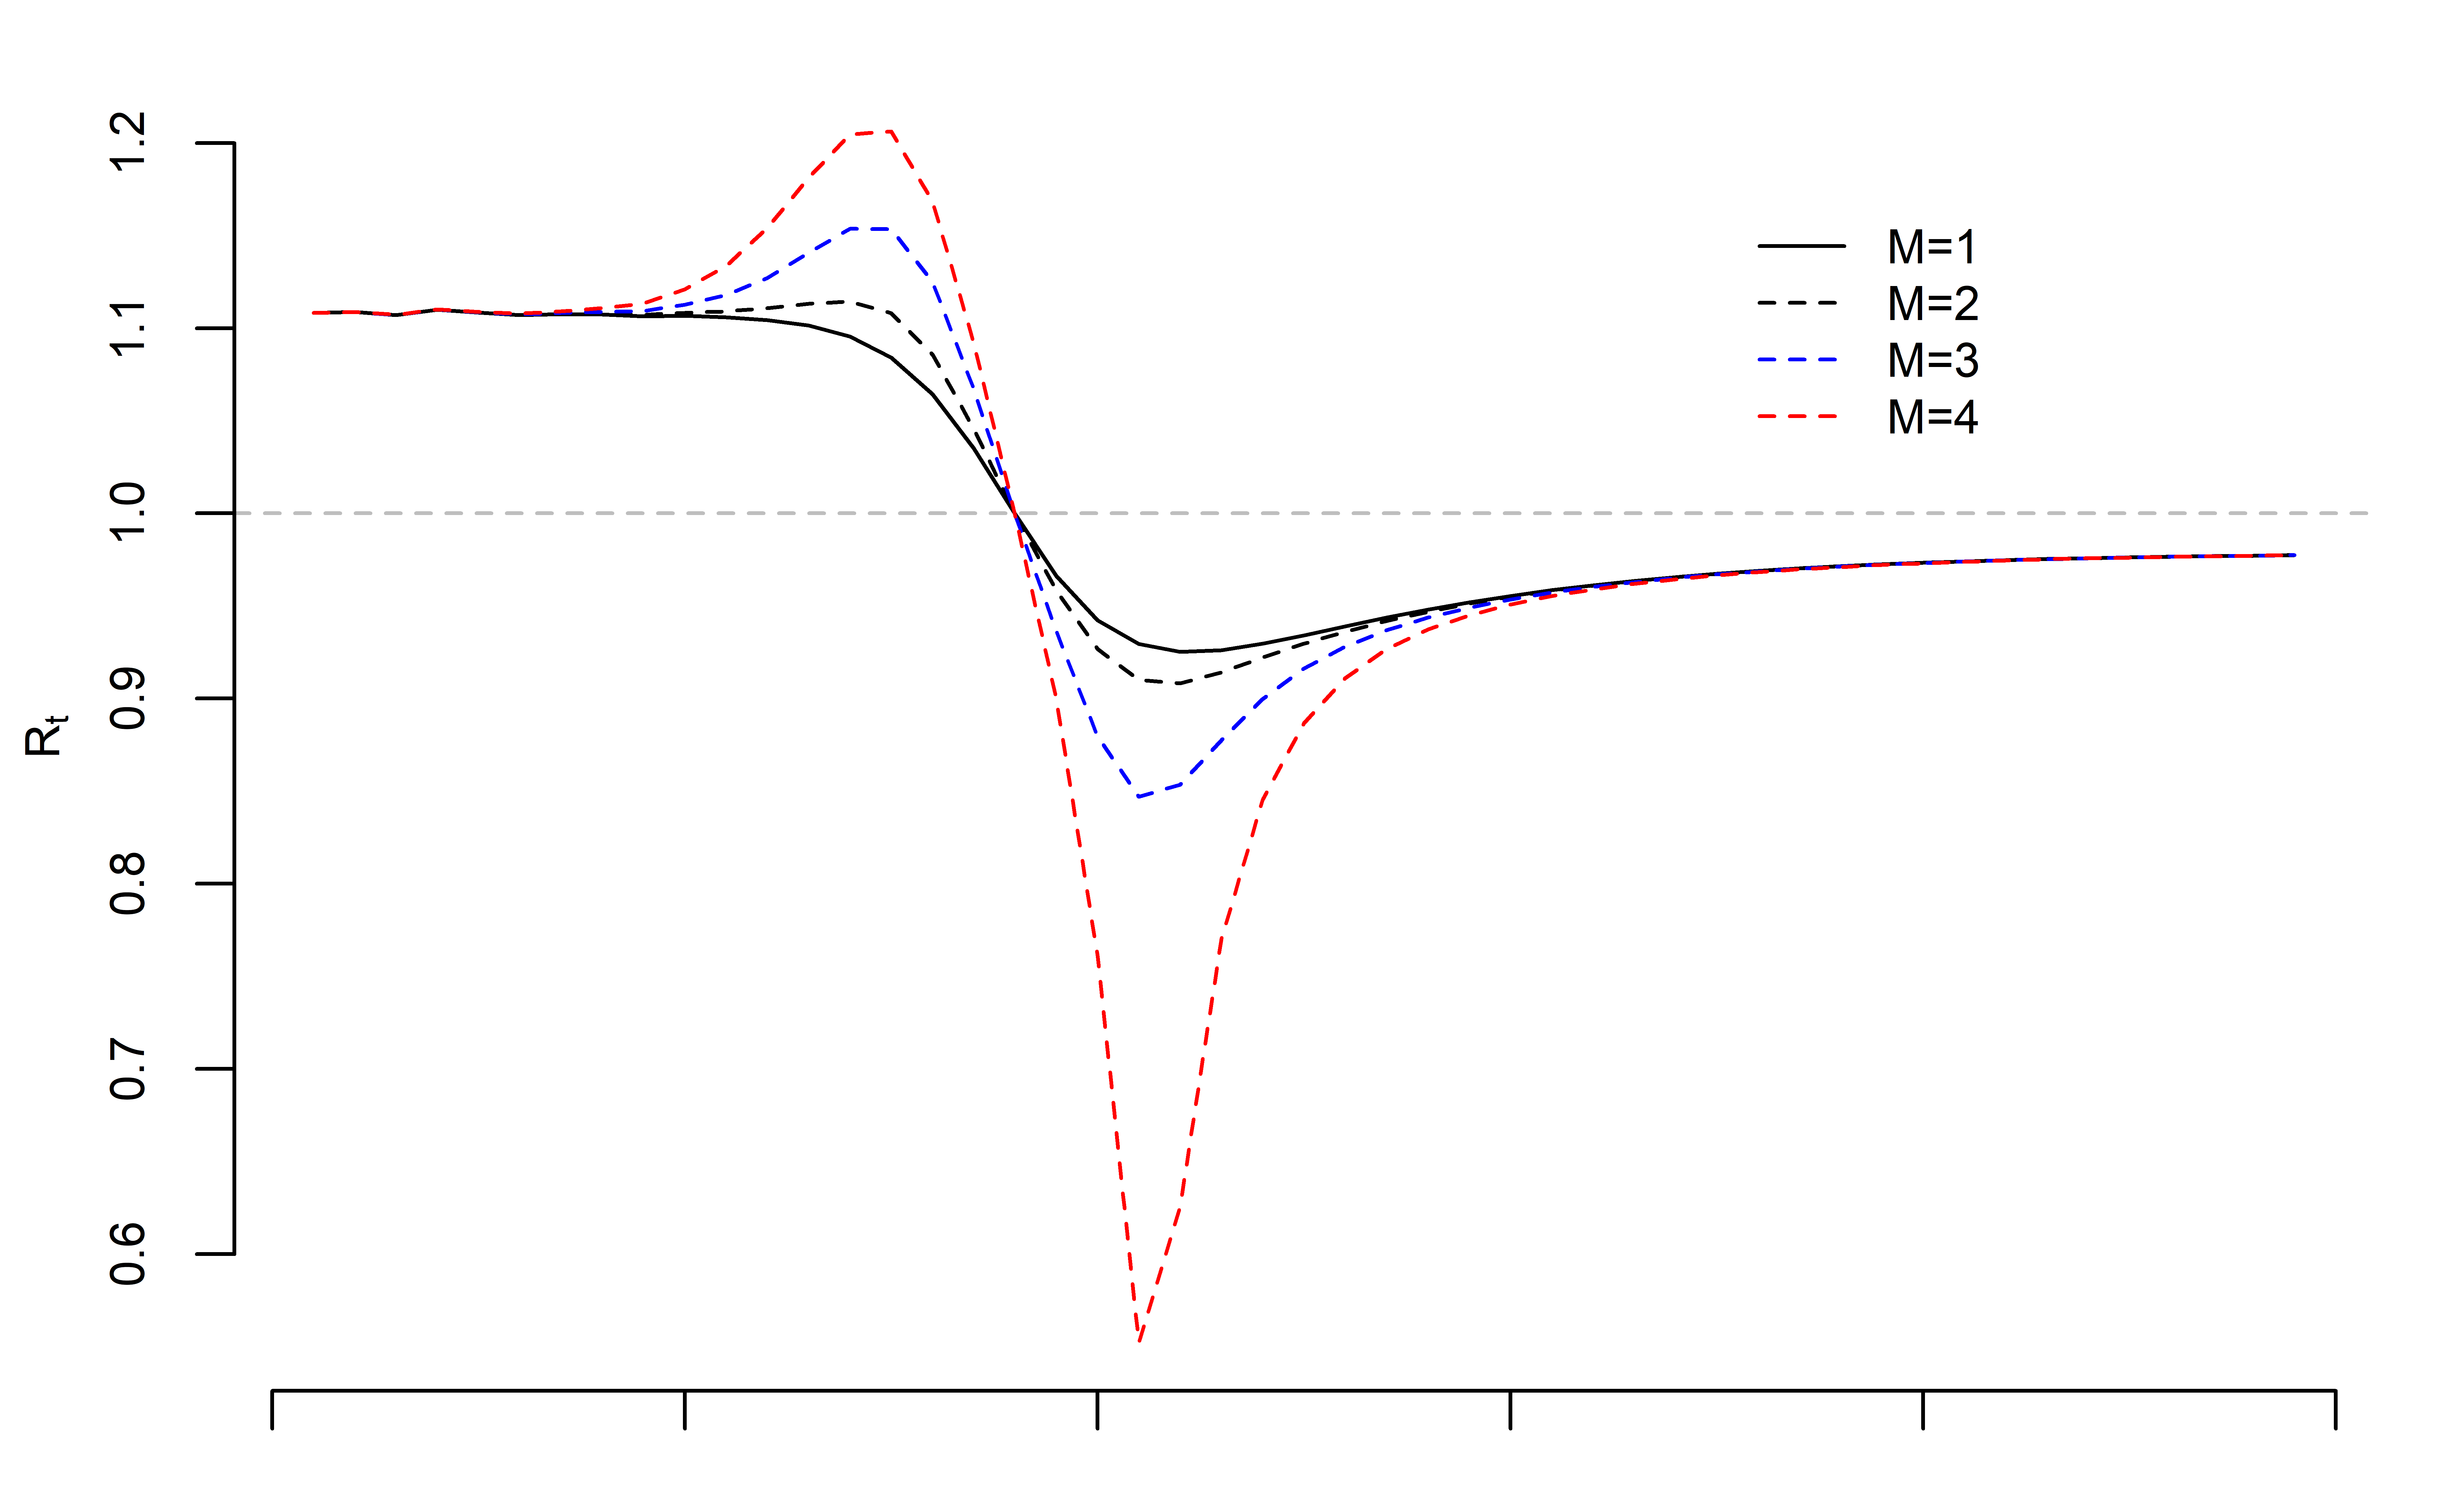
\includegraphics[width=.9\linewidth]{../methods/figs/sir_rt.png}
  \caption{A subfigure}
  \label{fig:sub2}
\end{subfigure}
\caption{A figure with two subfigures}
\label{fig:test}
\end{figure}

\subsection{Clinical trials}

Here we show how selection bias can even creep into clinical trial analysis. The key concern is whether clinical trials on COVID-19 recruit from the pool of individuals who have tested positive for COVID-19 or whether they sample randomly from the population, test, and then recruit from this subset of tested individuals.  To see this issue, suppose we have an outcome $Y$, a treatment $A$ and an \emph{unobserved} $U$.  Suppose treatment is assigned at random, i.e., $A =1$ with probability $50\%$ and $A=0$ with probability $50\%$.  Suppose the conditional mean of the outcome satisfies  $E(Y \mid U, A ) = \beta_0 + \beta_1 A + \beta_2 U + \beta_3 A U$.  Typically, we are interested in the \emph{causal effect} of $A$ on $Y$.  In counterfactual language,
$$
E( Y(A=1) - Y(A=0) ) = E_U ( E_A ( Y(A=1) - Y(A=0) \mid U=u ))
= \beta_1 + \beta_3 E(U).
$$
Even in a randomized experiment, the question is what the correct value for $E(U)$ is. For COVID-19, the value of interest is the expected value of $U$ in the population of COVID-19 positive individuals.  Due to selection bias, however, the bias in this marginal treatment effect compared to the true marginal effect of interest is $\beta_1 \cdot E_{\I} [ \rho_{I,U} ] \times \frac{f}{1-f} \times \sigma_U$.  Selection bias then leads to the estimated effect being biased if $\beta_1 \neq 0$.  Directionality of the bias will depend on the relationship between $U$ and $Y$.  If $U$ is a measure of disease severity, then it could be expected to see $\beta_1 > 0$ and therefore treatment effects to be overly optimistic as most individuals recruited are potentially higher on the severity index than the population average.

Randomization of treatment assignment in clinical trials negates unobserved confounders.  This, however, does not negate effect modifiers.  Therefore, for marginal treatment effects to be interpretable, there must be a well-defined population.  As our main interest is in causal effects on the population of COVID-19 positive.  Randomization within the clinical trial design yields internal validity, but we also need external validity to estimate the marginal effect correctly.

\section{Cross-population comparisons}

So far we have focused on understanding the limitations of using case-count data to understand population quantities of interest for a \emph{single} population (i.e., United States, Germany, France or Michigan, New York, London in isolation) at a single moment and over time.  Many are interested in cross-population comparisons.  Many pieces in the media as well as academic articles have plots of case-count over time aligned by time of first known case.  Others have claimed such comparisons unfair due to unequal population sizes and instead plotted case-count per million.  In this section, we focus on the statistical issues relevant to such comparisons. We do not make any comments on the multi-causal nature of success/failure in countries.

\subsection{Prevalence comparisons}

At a fixed time, suppose prevalence estimates $\bar y_1$ and $\bar y_2$ are observed for two populations. We can express $\bar y_1 - \bar y_2$ in statistical terms as
$$
(\bar Y_1 - \bar Y_2) + \left[ \rho_{I_1, Y_1} \times D_{M_1} \times \sqrt{\frac{1-f_1}{f_1}} \times \sigma_{Y_1}  - \rho_{I_2, Y_2} \times D_{M_2} \times \sqrt{\frac{1-f_2}{f_2}} \times \sigma_{Y_2} \right].
$$
The first term is the difference in population prevalence (i.e., the quantity of interest).  If random sampling were performed in each population, $E_{\I} [ \rho_{I_j, Y_j}] = 0$ and so the estimate would be unbiased.  However, the second term represents the complex error that results from selection bias.
The particular test of interest is $H_0: \bar Y_1 = \bar Y_2$.  Under the null, $\sigma_{Y_1} = \sigma_{Y_2}$.  In classical statistics, we would compute a Z-score:
$$
\begin{aligned}
\frac{\bar y_1 - \bar y_2}{ V_{SRS} (\bar y_1 - \bar y_2) } &=
\frac{\rho_{I_1, Y_1} \times D_{M_1} \times \sqrt{\frac{1-f_1}{f_1}}  - \rho_{I_2, Y_2} \times D_{M_2} \times \sqrt{\frac{1-f_2}{f_2}} }{ \sqrt{\frac{1}{N_1 -1} \times \frac{1-f_1}{f_1} + \frac{1}{N_2 - 1} \times \frac{1-f_2}{f_2}} }  \\
&\overset{\star}{=}
\sqrt{\frac{(N_1-1)(N_2 -1)}{N_1 + N_2}} \left[ \rho_{I_1, Y_1} - \rho_{I_2, Y_2} \right]
\end{aligned}
$$
Where the last equality holds under $f_1 = f_2$, i.e., same sampling rate relative to population size. This tells us that the exact error in the comparison of sample means, as an estimate of the difference in population means, scales as a function of the difference in data quality $\rho_{I_1, Y_1} - \rho_{I_2, Y_2}$ times a square root of a population adjustment.  For highly unequal population sizes (e.g., $N_1 \gg N_2$), the adjustment is approximated well by the square root of the smaller population size minus one (e.g. $\sqrt{N_2 -1}$).

\textcolor{red}{Take, for example, a comparison of the US and Canada.  The two population sizes are approximately 328 million and 38 million people.  Then the population adjustment is $5.84$ million. As of May 5th, Canada has performed a total of 24.92 tests per 1,000 people while the US has performed a total of 22.01 tests per 1,000 people (cite: https://ourworldindata.org/grapher/full-list-cumulative-total-tests-per-thousand)} so the data quantities are approximately equal to $f = 23/1000 = 0.023$.  Then, under a prevalence of 10\%, one would need the differential $\Delta_1-\Delta_2$ to be much smaller than $11.68 \times 10^{-6}$ in order for the selection bias to not impact.  So only under the very strong assumptions of equal data quantity and quality will the comparisons be valid and the $Z$-score can be treated as in the classical setting.  The issue is how to assess data quality equivalence among populations. \textcolor{red}{Discuss the measures in the literature.}  If this does not hold, then the width of the CIs need to be multipled by

\textcolor{red}{What is adjustment to CIs}.   Inserting the effective sample sizes can give us a better sense for a appropriate $Z$-score.  For example, using $n_eff = 20$ for each. And then
$$
Z_n = \frac{\bar y_1 - \bar y_2}{ \frac{1-f}{f} \sigma_y \sqrt{ \frac{1}{n_1 - 1} + \frac{1}{n_2 - 1}}}.
$$
So we see that we cannot reject the null. \textcolor{red}{We can do the same for different rates as well.}  This is not perfect but more appropriate.

\subsection{Case count comparisons}

We could instead think about the number of new cases $K_1$ and $K_2$ within each population.  Then
$$
y_1 - y_2 = \frac{N_1}{n_1} ( \bar y_1 - Y_{1}) + \left( \frac{N_1}{n_1} Y_{1} - \frac{N_2}{n_2} Y_2  \right).
$$
OK then we should compare relative counts?
The question is then ``What are you comparing at a populatoin level?''
$$
y_1/N_1 - y_2/ N_2 = \left[ f_1 \sigma_{Y_1} \rho_{I_1, Y_1} \sqrt{\frac{1-f_1}{f_1}} D_{M_1} - f_2 \sigma_{Y_2} \rho_{I_1, Y_1} \sqrt{\frac{1-f_1}{f_1}}  \right] + \left[ f_1 \bar Y_1 - f_2 \bar Y_2 \right]
$$
Is this a quantity of genuine interest? Under SRS, this makes sense if $f_1 = f_2$.  Otherwise, you are comparing apples and oranges.  With selection bias, it's not clear that agreement in this quantity is even desirable.

A final question is whether an observed drop in prevalence can be interpreted as a ``real'' decrease in prevalence.  To this end, one would typically construct a Z-score and perform a


$$
\frac{n}{N} \times \rho_{I,Y} \times \sqrt{\frac{1-f}{f}} \times \sigma_{Y} \times D_M
$$

\subsection{Rate comparisons}

An alternative is the comparison on the rates of case-count change over time.  Here, for simplicity, we focus on comparing the estimated effective reproductive rate.  We assume the two time-series are aligned so that $t=0$ is the time of first .  This negates the alignment issue and is common in the plots.

While the above issues on $Z$-scores and effective sample size are important, here we highlight a separate issue.  Namely, the interplay of bias when two trajectories when the peaks are slightly off.  We show that the biases can make us think the gap between two similar trajectories is larger than we would like!!!!
$$
R_{t1} - R_{t2} = \frac{1}{\gamma} \log \left( \frac{1 + e_{1t}}{1+e_{2t}} \right)
$$
where $e_{jt}$ is the error associated given in Section XX.  Recall that the error allowed for over-estimation prior to the peak and then under-estimation post-peak.  Here, these errors can mingle in interesting ways.  Consider two countries (A and B) in which the peak occurs 2 weeks prior for country A then country B but other.  Figure XX presents 1 week prior to the peak of A up to one week after the peak for country B.  Data for each country is simulated from an SIR model as described in Section XX.  We see that the errors interact in complex ways.  In week 1, the two countries appear the same; then in week 2, the gap between country A and B enlarges significantly as country A seems to see rapid improvement; then in week 3, country B improves and actually catches up to country A; then in month 4, country A sees rapid improvement while country B appears worse.  We are not claiming this is always the case, and indeed for small enough selection bias and/or large gaps in case-counts such complex behavior will not occur; however, this is simpy to point out how observed information can tell a more complex story than the truth (i.e., country A recovers 1 month prior to country B).

\begin{figure}
\centering
\begin{subfigure}{.5\textwidth}
  \centering
  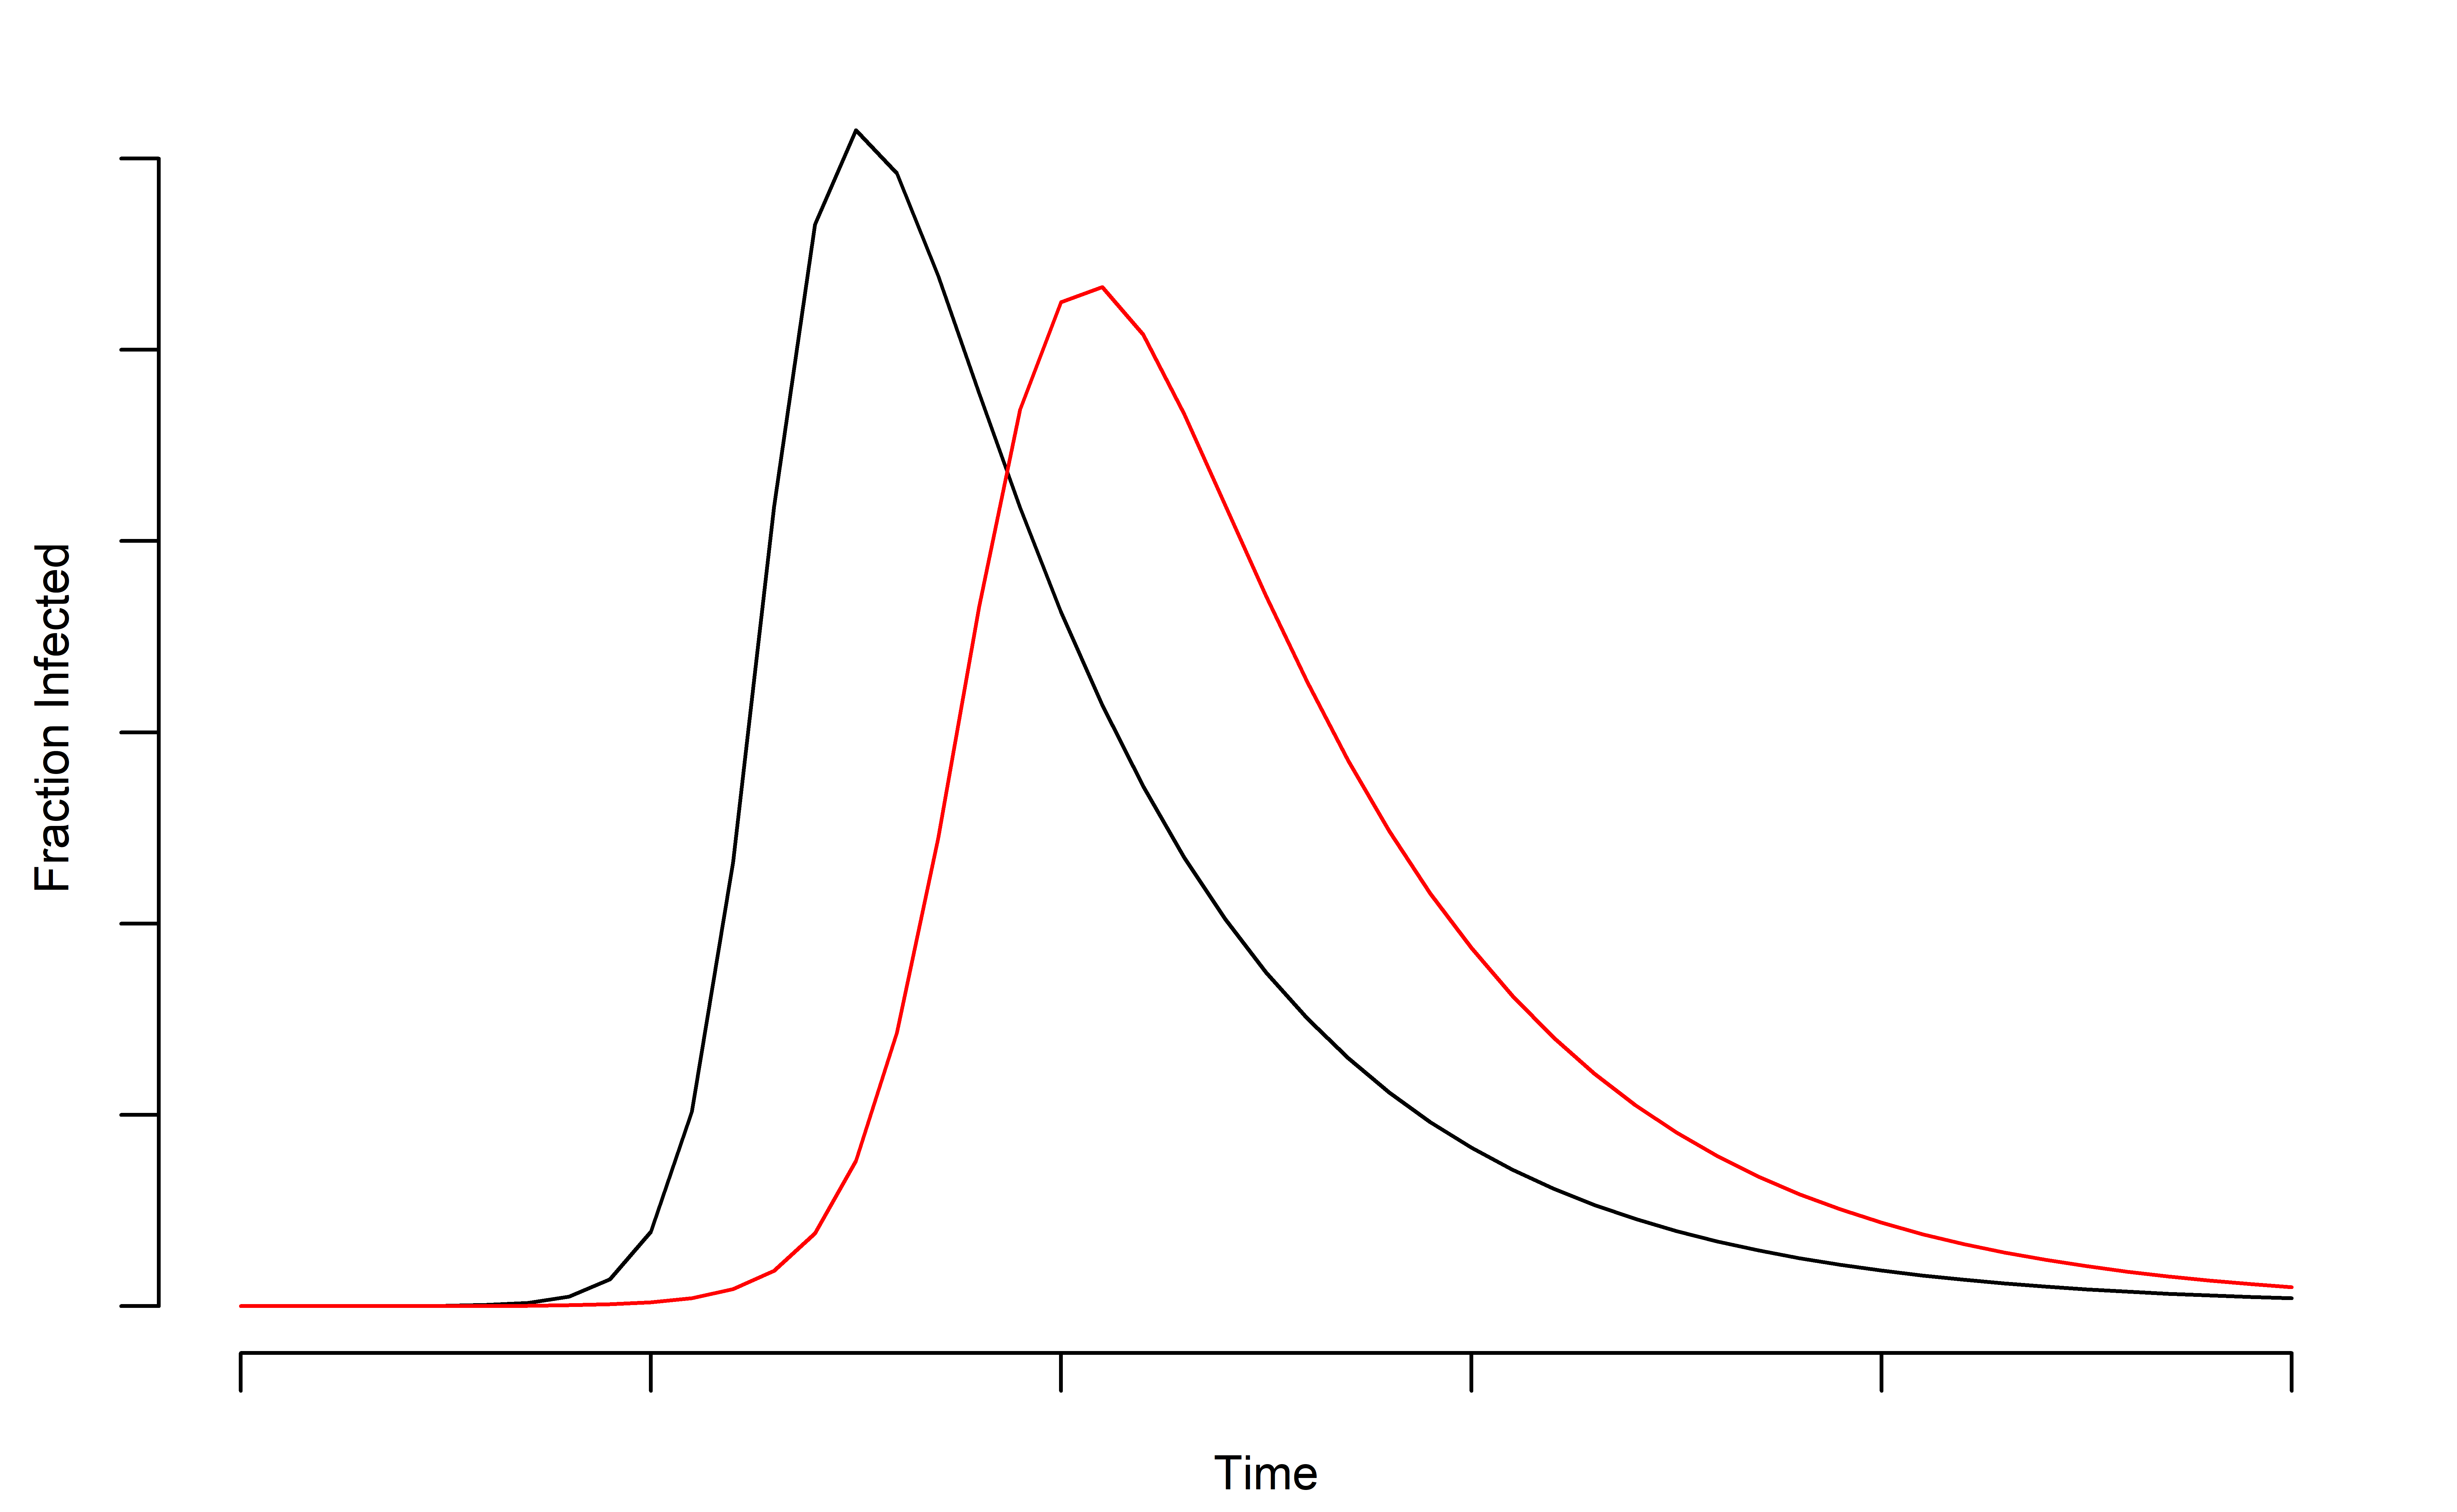
\includegraphics[width=.9\linewidth]{../methods/figs/sir.png}
  \caption{A subfigure}
  \label{fig:sub1}
\end{subfigure}%
\begin{subfigure}{.5\textwidth}
  \centering
  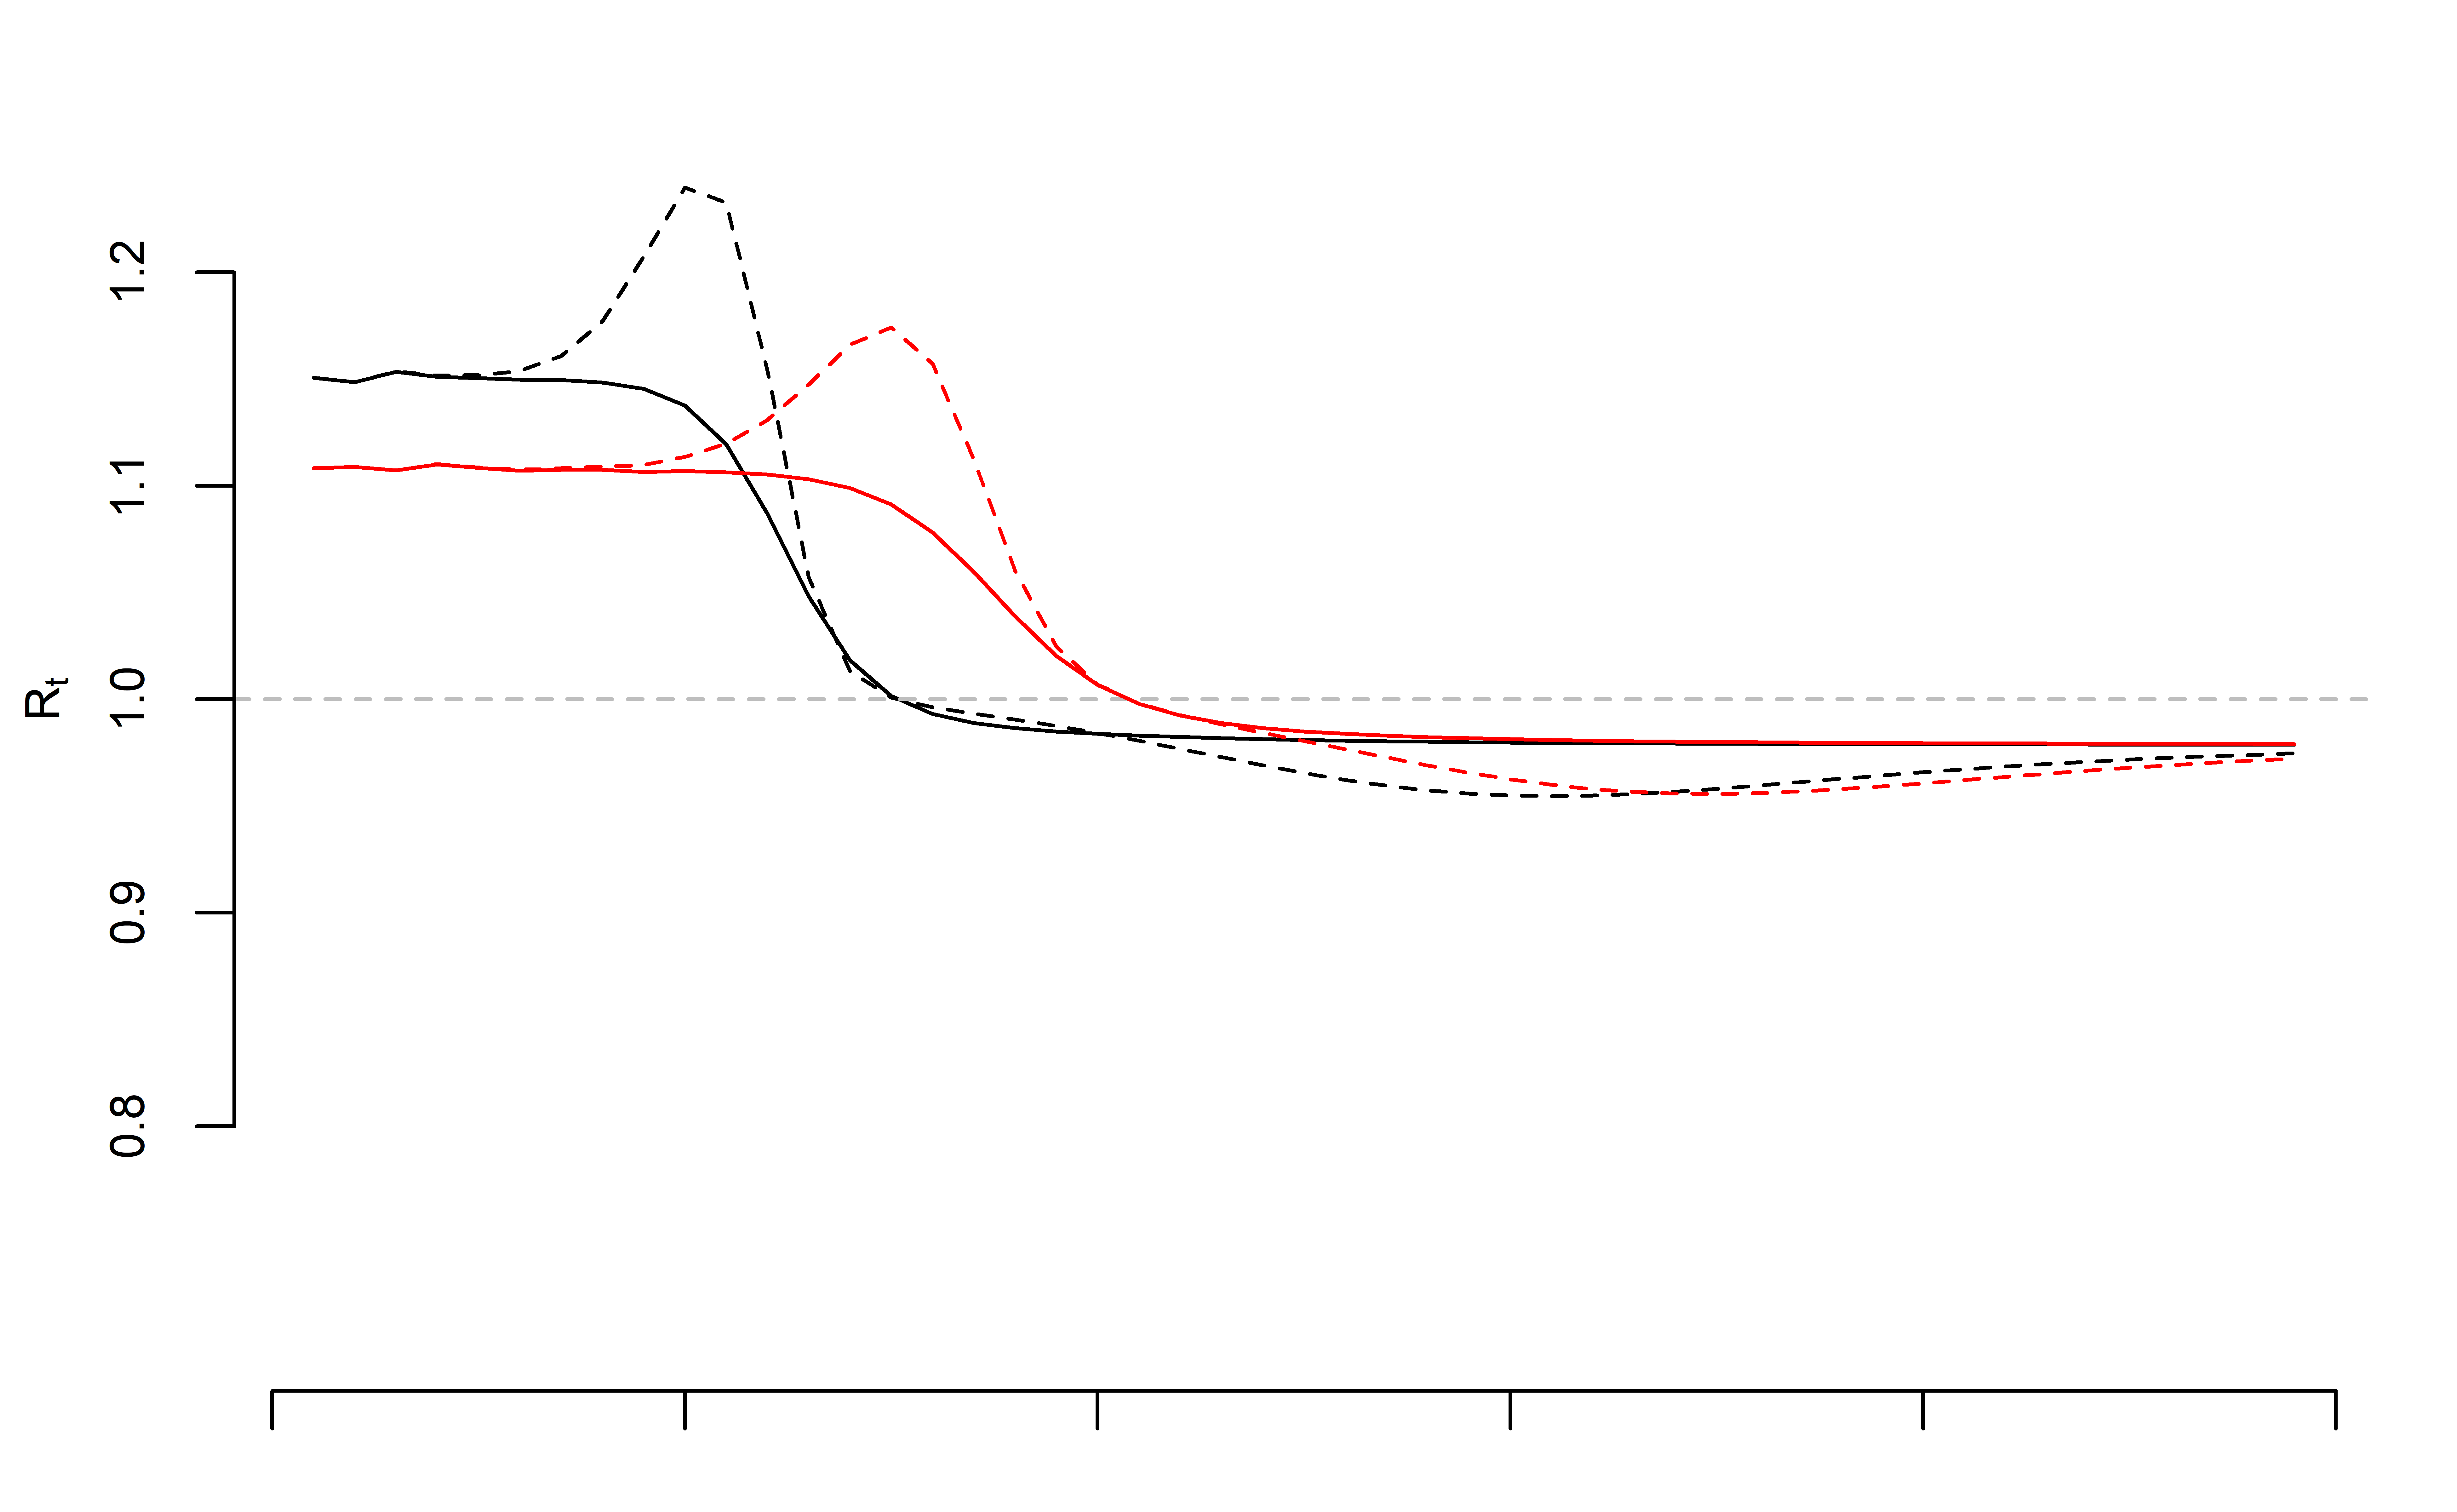
\includegraphics[width=.9\linewidth]{../methods/figs/sir_rt_comparison.png}
  \caption{A subfigure}
  \label{fig:sub2}
\end{subfigure}
\caption{A figure with two subfigures}
\label{fig:test}
\end{figure}

\subsection{Estimation of Data Quality}

Comparison of states with similar $f$ and similar testing inclusion protocols.  Not perfect.

\[
\rho = .004 \Rightarrow \Delta = 0.035 \times \sqrt{\frac{f \cdot (1-f)}{\bar Y \cdot (1 - \bar Y) }} = 0.00224 \Rightarrow M =
\]

We estimate $\rho$ using old and new methods.  Current SRS in US are weak.  So we just use my back of the envelope calculation. Tests per million as proxy since everyone is doing rationing. Cluster.


\subsection{Stratified setting}


\section{Stratified sampling: improving precision in low-prevalence environments}

Sampling network is hard.  Sampling high-risk strata is easy.  Simple example.
DTR and network connectivity is useful for understanding spread and where "testing should go".

Huge benefits when the rates are very different.

\section{Decision-making: data versus information.}

Above we point to flaws in using observed data to reason about the

\section{That which does not break us, makes us stronger (but potentially not smarter)}

A slightly altered version of Nietzsche's famous quote has become a mantra for post-pandemic thinking: \emph{That which which does not break us, makes us stronger}.  While potentially true via viral resistance, it is not clear that governments have yet to learn lessons on pandemic response.

During the current wave, understanding prevalence is key.  It helps us determine long-term risk for a community and make targeted interventions.  This will allow
When prevalence is below a certain threshold, we can return to daily life.

Once we ``return to normal''\footnote{or at least the new normal}, it is clear that testing strategies should focus on early detection, heading off future outbreaks.
\emph{Anyone who wishes to go back to work}.  While laudable, without complete compliance, we may be riddles with selection bias and measurement-error.  This ignores even the practical and ethical quandaries of how to .

What do we do when we are faced with?  We design experiments with our objectives in mind.

(A) Prevalence: Targeted shutdowns
(B) Risk Detection: Contact tracing and altering

Use prior results to show that ratio estimator under SRS is a good predictor of potential outbreak.

``Disease free''


\section{Discussion}

In current crisis, data quality is tied to data quantity due to rationing system. \emph{Testing }
Increasing testing under test rationing lowers correlation.  Example in Michigan and try and find CA and NY numbers.  Then show that this may cause higher FPs (cite antibody studies).

Plot Michigan tests per million and positives.  Next to NY.  Both as of April moved to prioritized sampling for symptomatic individuals.

There is a lot of hidden information in the selection indicator $I_j$.  Up until recently, an individual had to first \emph{want} to be tested, then call their primary health care provider who decided whether they met thresholds for testing

. Currently, we are unaware of reliable information on the number of cases where

In the UU
We assume that the percentage of tests is rationed according to severity of symptoms.

Note that a person who displays severe symptoms may be COVID negative.  This gives us a sense of the data quality.

\emph{Increasing testing leads to lower correlation only if we see the gap $\Delta$ decrease.  If we just see $f$ }

The CDC reports 413,867 total tests performed in the US as of April 25th.




Use of these bounds as E-scores.  How bad can it go?

Interventions in this area are designed experiments.  Unlike Fischer's null, here the objectives are settings, statisticians.

Account for data quality in models by incorporating auxiliary information.  Perform advanced sensitivity analysis.  Forecasts should be called coutnerfactual forecasts.

Poststratifiers and systematic measurement error.

A critical question is whether there are alternative data streams that may be leveraged to understand the handling of the COVID-19 pandemic in the US.

\appendix

\section{Imperfect testing: derivation}

We considered the mean estimator
$$
\bar y_n^\star = \frac{\sum_{j=1}^N Y_j^\star I_j}{\sum_{j=1}^N I_j} = \frac{\sum_{i=1}^N  I_j Y_j^\star }{\sum_{j=1}^N  I_j } = \frac{\sum_{i=1}^N  I_j \left[ Y_j (1-P_j) + (1-Y_j) P_j \right]}{\sum_{j=1}^N  I_j }
$$
For any set of numbers $\{ A_1, \ldots, A_N \}$ we can view it as the support of a random variable $A_J$ induced by the random index $J$ defined on $\{1,\ldots, N\}$.  When $J$ is uniformly distributed $E_J (A_J) = \sum_{j=1}^N A_j / N \equiv \bar A_N$. Then
$$
\begin{aligned}
\bar y_n^\star  - \bar Y_N &= \frac{E_J \left[ I_J \left[ Y_J (1-P_J) + (1-Y_J) P_J \right] \right]}{E_J [ I_J ] } - E_J[Y_J] \\
&= \frac{E_J \left[ I_J P_J (1-2Y_J) \right]}{E_J [ I_J ] } + \left( \frac{E_J [I_J Y_J]}{E_J [ I_J ] } - \frac{E_J[Y_J] E_J[I_J]}{E_J[I_J]} \right) \\
\end{aligned}
$$
The term in parentheses can be re-written as
$$
\begin{aligned}
\frac{E_J [I_J Y_J]- E_J[Y_J] E_J[I_J]}{E_J[I_J]} &=  \frac{E_J [I_J Y_J]- E_J[Y_J] E_J[I_J]}{\sqrt{V_J(I_J) V_J(Y_J)}} \frac{\sqrt{V_J(I_J)}}{E_J[I_J]} \times \sqrt{V_J(Y_J)} \\
&= \rho_{I,Y} \times \sqrt{\frac{(1-f)}{f}} \times \sigma_Y
\end{aligned}
$$
which agrees with Meng's (2019) decomposition. For the other term, first we define $Z_j := 1 - 2 Y_j $. Then $Z_j = 1$ if $Y_j = 0$ and $Z_j = -1$ if $Y_j = 1$. Then the term can be re-written as
$$
\begin{aligned}
\frac{E_J \left[ I_J P_J (1-2Y_J) \right]}{E_J [ I_J ] } &= \left( \frac{E_J \left[ I_J P_J Z_J \right]}{E_J [ I_J ] } -  \frac{E_J \left[ P_J Z_J \right] E_J[ I_J]}{E_J [ I_J ] } \right) +  \frac{E_J \left[ P_J Z_J \right] E_J[ I_J]}{E_J [ I_J ] } \\
\end{aligned}
$$
The term in parentheses can be re-expressed using the previous technique as:
$$
\rho_{I, PZ} \times \sqrt{\frac{1-f}{f}} \times \sigma_{PZ}
$$
where now the ``data defect'' and ``problem difficulty'' are with respect to $PZ$ rather than $Y$. The final term is equal to
$$
\begin{aligned}
E_J [P_J Z_J ] &= E_J [ E_J [ P_J Z_J \mid Y_J ] ] \\
&= \pr (P = 1 \mid Y = 0) (1-\bar Y) - \pr(P=1 \mid Y = 1) \bar Y \\
&= FP - (FP + FN) \cdot \bar Y
\end{aligned}
$$
Combining these yields:
$$
\bar y_n^\star - \bar Y = \sqrt{\frac{1-f}{f}} \left[\rho_{I,Y} \sigma_Y + \rho_{I, PZ} \sigma_{PZ} + \sqrt{\frac{f}{1-f}} \left( FP - (FP+FN) \bar Y \right) \right]
$$
For the binary outcome $Y$, we have $\sigma_Y = \sqrt{\bar Y (1-\bar Y)}$. Moreover,
$$
\begin{aligned}
V_J(P_J Z_J) &= E_J[(P_J Z_J)^2] - E[P] E[Z] \\
&= E[P] - E[P] (1 - 2 \bar Y) = 2 \bar Y E_J [ P_J ] \\
&= 2 \bar Y \left( FP (1-\bar Y) + FN \bar Y \right) \\
\Rightarrow \sigma_{PZ} &= \sqrt{ 2 \bar Y \left( FP (1-\bar Y) + FN \cdot  \bar Y \right) }
\end{aligned}
$$
Then the formula for the error is given by:
$$
\sqrt{\frac{1-f}{f}} \left[\rho_{I,Y} \sqrt{\bar Y (1-\bar Y)} + \rho_{I, PZ} \sqrt{ 2 \bar Y \left( FP (1-\bar Y) + FN \cdot \bar Y \right )} + \sqrt{\frac{f}{1-f}} \left( FP - (FP+FN) \bar Y \right) \right]
$$

\subsection{Simple cases}

We consider two simple cases here.  First, we assume no false positive results, i.e., set $FP=0$.  Then $\sigma_{PZ} = \bar Y \sqrt{2 FN}$.  Then the math simplifies:
$$
\bar y_n^\star - \bar Y = \bar Y \sqrt{\frac{1-f}{f}} \left[\rho_{I,Y} \sqrt{\frac{1-\bar Y}{\bar Y}} + \sqrt{FN} \left( \sqrt{2} \rho_{I, PZ} - \sqrt{\frac{f}{1-f}} \sqrt{FN} \right)  \right]
$$
The sign of the error therefore depends on true data quality ($\rho_{I, Y}$), odds ratio, observed data quality~$\rho_{I,PZ}$, false negative rates (FN), and sample fraction $f$.

Second, we assume no false negative results, i.e., set $FN=0$.  Then $\sigma_{PZ} = \sqrt{2 FP \bar Y (1-\bar Y)}$.  Then the math simplifies:
$$
\bar y_n^\star - \bar Y = \sqrt{\bar Y (1-\bar Y)} \sqrt{\frac{1-f}{f}} \left[\rho_{I,Y} +  \sqrt{FP} \left( \sqrt{2} \rho_{I, PZ} + \sqrt{\frac{f}{1-f}} \sqrt{FP} \sqrt{1-\bar Y} \right)  \right]
$$
The sign of the error therefore depends on true data quality ($\rho_{I, Y}$),  observed data quality~$\rho_{I,PZ}$, false positive rates (FP), one minus prevalence ($1-\bar Y$), and sample fraction $f$.

\subsection{Adjusted estimator}

Define $\bar y_n^{\star \star} = \bar y_n^\star + FN \bar y_n^\star - FP(1-\bar y_n^\star)$; then the error is
$$
\bar y_n^{\star \star} - \bar Y = \sqrt{\frac{1-f}{f}} \left[ \rho_{I, Y} \sigma_{Y} (1+FP+FN)  + \rho_{I, PZ} \sqrt{ 2 \bar Y \left( FP (1-\bar Y) + FN \bar Y \right)} \right]
$$
In the case when false negative rate is zero, we have
$$
\bar y_n^{\star \star} - \bar Y = \sqrt{\frac{1-f}{f}} \sqrt{\bar Y(1-\bar Y)} \left[ \rho_{I, Y} (1+FP) + \rho_{I, PZ} \sqrt{ 2 FP } \right]
$$
In the case when false positive rate is zero, we have
$$
\bar y_n^{\star \star} - \bar Y = \sqrt{\frac{1-f}{f}} \sqrt{\bar Y(1-\bar Y)} \left[ \rho_{I, Y} (1+FN) + \rho_{I, PZ} \sqrt{ 2 FN } \times \sqrt{\frac{\bar Y}{1-\bar Y}} \right]
$$


\subsection{Estimate of observed data quality}

$$
\begin{aligned}
\rho_{I,PZ} &= \frac{C(I, PZ)}{\sqrt{V(PZ) V(I)}} \\
&= \frac{C(I, PZ)}{\sqrt{V(Y) V(I)}} \sqrt{\frac{V(Y)}{V(PZ)}} \\
&= \rho_{I,Y} \frac{C(I,PZ)}{C(I,Y)} \sqrt{ \frac{(1-\bar Y)}{2 ( FP (1-\bar Y) + FN \cdot \bar Y)} }
\end{aligned}
$$

$$
\begin{aligned}
C(I, PZ) &= E[ I P Z ] - E[I] E[PZ] \\
&=  [FP f_0 - (FP f_0 + FN f_1) \bar Y] - f [ FP - (FP+FN) \bar Y ] \\
&=  - FP \Delta \bar Y + FP \bar Y^2 \Delta - FN \bar Y^2 \Delta \\
&=  - \Delta \bar Y (FP \cdot (1-\bar Y) + FN \cdot \bar Y) \\
\end{aligned}
$$
where $f = f_1 \bar Y + f_0 (1-\bar Y)$ so $f_0 - f = -\Delta \bar Y$ and $f_1 - f = \Delta (1-\bar Y)$.
$$
\begin{aligned}
C(I, Y) &= E[ I Y ] - f \bar Y \\
&=  f_1 \bar Y + f_0 (1-\bar Y) - f \bar Y \\
&=  f_0 (1-\bar Y) + \Delta (1-\bar Y) \bar Y \\
&= (1-\bar Y) (f_0 + \Delta \bar Y)
\end{aligned}
$$
Combining yields
$$
\begin{aligned}
\rho_{I,PZ} &= \rho_{I,Y} \times \frac{- \Delta \bar Y (FP \cdot (1-\bar Y) + FN \cdot \bar Y) }{(1-\bar Y) (f_0 + \Delta \bar Y)} \times \sqrt{ \frac{(1-\bar Y)}{2 ( FP (1-\bar Y) + FN \cdot \bar Y)} } \\
&= - \rho_{I, Y} \times \Delta \times \sqrt{\frac{\bar Y}{1-\bar Y}} \frac{\sqrt{FP(1-\bar Y) + FN \cdot \bar Y}}{f_0 (1-\bar Y) + f_1 \bar Y} \times \sqrt{\frac{\bar Y}{2}}
\end{aligned}
$$
We can then re-write $\rho_{I,Y} \sigma_Y + \rho_{I,PZ} \sigma_{PZ}$ as
$$
\rho_{I,Y} \sigma_Y \left( 1 - \Delta \times \frac{\bar Y}{1-\bar Y} \times \frac{FP(1-\bar Y) + FN \cdot \bar Y}{f_0 (1-\bar Y) + f_1 \bar Y} \right)
$$
Suppose $f_1 = M \cdot f_0$.  Then $\Delta = f_1 - f_0 = f_0 (M-1)$ and $f_0 (1-\bar Y) + f_1 \bar Y = f_0 ( (1-\bar Y) + M \bar Y )$ and we can re-write above as
$$
\rho_{I,Y} \sigma_Y \left( 1 - (M-1) \times \frac{\bar Y}{1-\bar Y} \times \frac{FP(1-\bar Y) + FN \cdot \bar Y}{(1-\bar Y) + M \bar Y} \right).
$$

\subsection{Ratio estimator}

Let ${\bf u} = (u_1,u_2) \in \mathbb{R}^2$ and $g({\bf u}) = \frac{u_2}{u_1}$, i.e., a differentiable function $g:\mathbb{R}^2 \to \mathbb{R}$. Centering a Taylor series expansion of second-order around coordinates $(U_2, U_1) \in \mathbb{R}^2$ yields
$$
\begin{aligned}
g({\bf u}) =& g(U_1, U_2) - \frac{U_2}{U_1^2} (u_1 - U_1) + \frac{1}{U_1} (u_2 - U_2) \\
&+ \frac{1}{2} \left[ \frac{2 U_2}{U_1^3} (u_1 - U_1)^2 + 0 \times (u_2 - U_2)^2 - 2 \times (u_1 - U_1) (u_2 - U_2) \frac{1}{U_1^2} \right]
\end{aligned}
$$
Plugging in $(\bar y_1, \bar y_2)$ for $(u_1, u_2)$ and $(\bar Y_1, \bar Y_2)$ for $(U_1, U_2)$ yields
$$
\begin{aligned}
\frac{\bar y_2}{\bar y_1} - \frac{\bar Y_2}{\bar Y_1} =& - \frac{\bar Y_2}{\bar Y_1^2} (\bar y_1 - \bar Y_1) + \frac{1}{\bar Y_1} (\bar y_2 - \bar Y_2) \\
&+ \frac{\bar Y_2}{\bar Y_1^3} (\bar y_1 - \bar Y_1)^2 -  (\bar y_1 - \bar Y_1) (\bar y_2 - \bar Y_2) \frac{1}{\bar Y_1^2} \\
&= \frac{\bar Y_2}{\bar Y_1} \bigg[  \rho_{I_2,Y_2} \sqrt{\frac{1-f_2}{f_2}} CV (Y_2)  -\rho_{I_1,Y_1} \sqrt{\frac{1-f_1}{f_1}} CV (Y_1) \\
&+ \rho^2_{I_1,Y_1} \frac{1-f_1}{f_1} CV^2 (Y_1) -  \rho_{I_1,Y_1} \sqrt{\frac{1-f_1}{f_1}} CV (Y_1) \times \rho_{I_2,Y_2} \sqrt{\frac{1-f_2}{f_2}} CV (Y_2)   \bigg] \\
&= \frac{\bar Y_2}{\bar Y_1} \bigg[ \rho_{I_2,Y_2} \sqrt{\frac{1-f_2}{f_2}} CV (Y_2)  -\rho_{I_1,Y_1} \sqrt{\frac{1-f_1}{f_1}} CV (Y_1) \bigg] \left[ 1 - \rho_{I_1,Y_1} \sqrt{\frac{1-f_1}{f_1}} CV (Y_1) \right]
\end{aligned}
$$
where the second equality is obtained by plugging in the statistical decomposition of the error for both time points and the coefficient of variation being defined as $CV(Y) := \sigma_Y/\mu_Y$.  Under measurement-error, the extra terms $D_{2}$ and $D_1$ can be inserted in the correct locations.

\section{Derivation for the effective sample size}

\begin{equation} \label{eq:binaryrho}
\rho_{I,Y} = \Delta \sqrt{\frac{\bar Y (1 - \bar Y)}{f (1-f)} }
\end{equation}
where $\Delta = P_J (I_J = 1 \mid Y_J = 1) - P(I_J = 1 \mid Y_J = 0)$.  Suppose that $\Delta = 10\%$ and $\bar Y = 10\%$ then $\rho_{I,Y}$ is given by
We expect the correlation to be more on the order



\section{Quotes}

I prefer to think of a statistical sensibility rather than statistical thinking. It’s “less than an agenda but more than an attitude.”  It allows for methodological preference while avoiding dogma. Paired with data analytic humility and I think you have proper “data science”

“Routine statistical questions are less common than questionable statistical routines...” McCullagh (2005).

If an issue can be addressed nonparametrically then it will often be better to tackle it parametrically; however, if it cannot be resolved nonparametrically then it is usually dangerous to resolve it parametrically.” (p.96)

A test of meaningfulness of a possible model for a data-generating process is whether it can be used directly to simulate data.” (p.104).  In our current setting, this most certainly related to simulation while accounting for measruement error.




\end{document}